\documentclass{beamer}
\usepackage[utf8]{inputenc}
\usetheme{Madrid}
\usecolortheme{default}
\usepackage{amsmath,amssymb,amsfonts,amsthm}
\usepackage{txfonts}
\usepackage{tkz-euclide}
\usepackage{listings}
\usepackage{adjustbox}
\usepackage{array}
\usepackage{tabularx}
\usepackage{gvv}
\usepackage{lmodern}
\usepackage{circuitikz}
\usepackage{tikz}
\usepackage{graphicx}

\setbeamertemplate{page number in head/foot}[totalframenumber]

\usepackage{tcolorbox}
\tcbuselibrary{minted,breakable,xparse,skins}



\definecolor{bg}{gray}{0.95}
\DeclareTCBListing{mintedbox}{O{}m!O{}}{%
  breakable=true,
  listing engine=minted,
  listing only,
  minted language=#2,
  minted style=default,
  minted options={%
    linenos,
    gobble=0,
    breaklines=true,
    breakafter=,,
    fontsize=\small,
    numbersep=8pt,
    #1},
  boxsep=0pt,
  left skip=0pt,
  right skip=0pt,
  left=25pt,
  right=0pt,
  top=3pt,
  bottom=3pt,
  arc=5pt,
  leftrule=0pt,
  rightrule=0pt,
  bottomrule=2pt,
  toprule=2pt,
  colback=bg,
  colframe=orange!70,
  enhanced,
  overlay={%
    \begin{tcbclipinterior}
    \fill[orange!20!white] (frame.south west) rectangle ([xshift=20pt]frame.north west);
    \end{tcbclipinterior}},
  #3,
}
\lstset{
    language=C,
    basicstyle=\ttfamily\small,
    keywordstyle=\color{blue},
    stringstyle=\color{orange},
    commentstyle=\color{green!60!black},
    numbers=left,
    numberstyle=\tiny\color{gray},
    breaklines=true,
    showstringspaces=false,
}
%------------------------------------------------------------
%This block of code defines the information to appear in the
%Title page
\title %optional
{5.13.2}

%\subtitle{A short story}

\author % (optional)
{BALU-ai25btech11017}



\begin{document}


\frame{\titlepage}
\begin{frame}{Question}
Find the equation of the circle having $(1,-2)$ as its centre and passing through the intersection of 
\begin{align}
3x + y = 14, \quad 2x + 5y = 18.
\end{align}
\\ 
\end{frame}
\begin{frame}{Theoretical Solution}
Let us solve the given equation theoretically and then verify the solution computationally \\
According to the question, \\
\begin{align}
   \myvec{3&&1\\2&&5}\vec{B}=\myvec{14\\18}\\
   \vec{B}=\myvec{4\\2}
\end{align}
circle equation is\\
\begin{align}
   \vec{x}\vec{x}^T+2\vec{u}^T\vec{x}+f=0\\
   \vec{u}=\myvec{1\\-2}\
\end{align}
\end{frame}
\begin{frame}{Theoretical Solution}
point $\vec{B}$ lies on circle,so
\begin{align}
    \vec{b}\vec{b}^T+2\vec{u}^T\vec{b}+f=0\\
    f=-20\
\end{align}
hence the requried circle equation is
\begin{align}
    \vec{x}\vec{x}^T+2\myvec{1&&-2}\vec{x}-20=0\
\end{align}
\end{frame}
\begin{frame}[fragile]
    \frametitle{C Code}

    \begin{lstlisting}
  #include <stdio.h>
#include <math.h>

int main() {
    // Circle centre
    double h = 1, k = -2;

    // Solve intersection of 3x + y = 14  and  2x + 5y = 18
    // Equation 1: 3x + y = 14  --> y = 14 - 3x
    // Substitute in 2x + 5y = 18
    double x, y;
    x = (18 - 5*14) / (2 - 15);   // Simplified from substitution
    y = 14 - 3*x;

    // Radius = distance between (h,k) and intersection point
    double r = sqrt(pow(x - h, 2) + pow(y - k, 2));

  

    \end{lstlisting}
\end{frame}
\begin{frame}[fragile]
    \frametitle{C Code }
    \begin{lstlisting}
  // Print results
    printf("Intersection Point: (%.2f, %.2f)\n", x, y);
    printf("Centre: (%.2f, %.2f)\n", h, k);
    printf("Radius: %.2f\n", r);
    printf("Equation of Circle: (x - %.2f)^2 + (y - %.2f)^2 = %.2f^2\n", h, k, r);

    return 0;
}
    \end{lstlisting}
\end{frame}
\begin{frame}[fragile]
    \frametitle{python Code }
    \begin{lstlisting}
#Code by GVV Sharma (modified for circle through line intersection)
#Sep 27, 2025
#Released under GNU GPL

import sys
import numpy as np
import matplotlib.pyplot as plt
from numpy import linalg as LA

# Local imports from CoordGeo
sys.path.insert(0, '/sdcard/github/matgeo/codes/CoordGeo')
from line.funcs import line_isect, line_norm
from conics.funcs import circ_gen

# Line equations: 3x + y = 14,  2x + 5y = 18
n1 = np.array([3,1]).reshape(-1,1)
c1 = 14





  \end{lstlisting}
\end{frame}
\begin{frame}[fragile]
    \frametitle{python Code }
    \begin{lstlisting}
n2 = np.array([2,5]).reshape(-1,1)
c2 = 18

# Intersection of lines
P = line_isect(n1,c1,n2,c2)

# Circle centre
O = np.array([1,-2]).reshape(-1,1)

# Radius = distance between centre and intersection point
r = LA.norm(O-P)

# Generate circle
x_circ = circ_gen(O,r)

# Generate lines
x_line1 = line_norm(n1,c1,-5,5)
x_line2 = line_norm(n2,c2,-5,5)

\end{lstlisting}
\end{frame}
\begin{frame}[fragile]
    \frametitle{python Code }
    \begin{lstlisting}
# Plotting
plt.plot(x_circ[0,:], x_circ[1,:], label="Circle")
plt.plot(x_line1[0,:], x_line1[1,:], label="$3x+y=14$")
plt.plot(x_line2[0,:], x_line2[1,:], label="$2x+5y=18$")

# Points
plt.scatter(P[0],P[1],color='red')
plt.scatter(O[0],O[1],color='blue')
plt.annotate("Intersection P",(P[0],P[1]),textcoords="offset points",xytext=(10,10))
plt.annotate("Centre O",(O[0],O[1]),textcoords="offset points",xytext=(10,-10))


    \end{lstlisting}
\end{frame}
\begin{frame}[fragile]
    \frametitle{python Code }
    \begin{lstlisting}
# Axes formatting
ax = plt.gca()
ax.spines['top'].set_color('none')
ax.spines['right'].set_color('none')
ax.spines['left'].set_position('zero')
ax.spines['bottom'].set_position('zero')
plt.legend()
plt.grid()
plt.axis("equal")

# Save and show
plt.savefig("circle_question.png", dpi=300)
plt.show()
     \end{lstlisting}
\end{frame}
\begin{frame}{Plot}
    \centering
    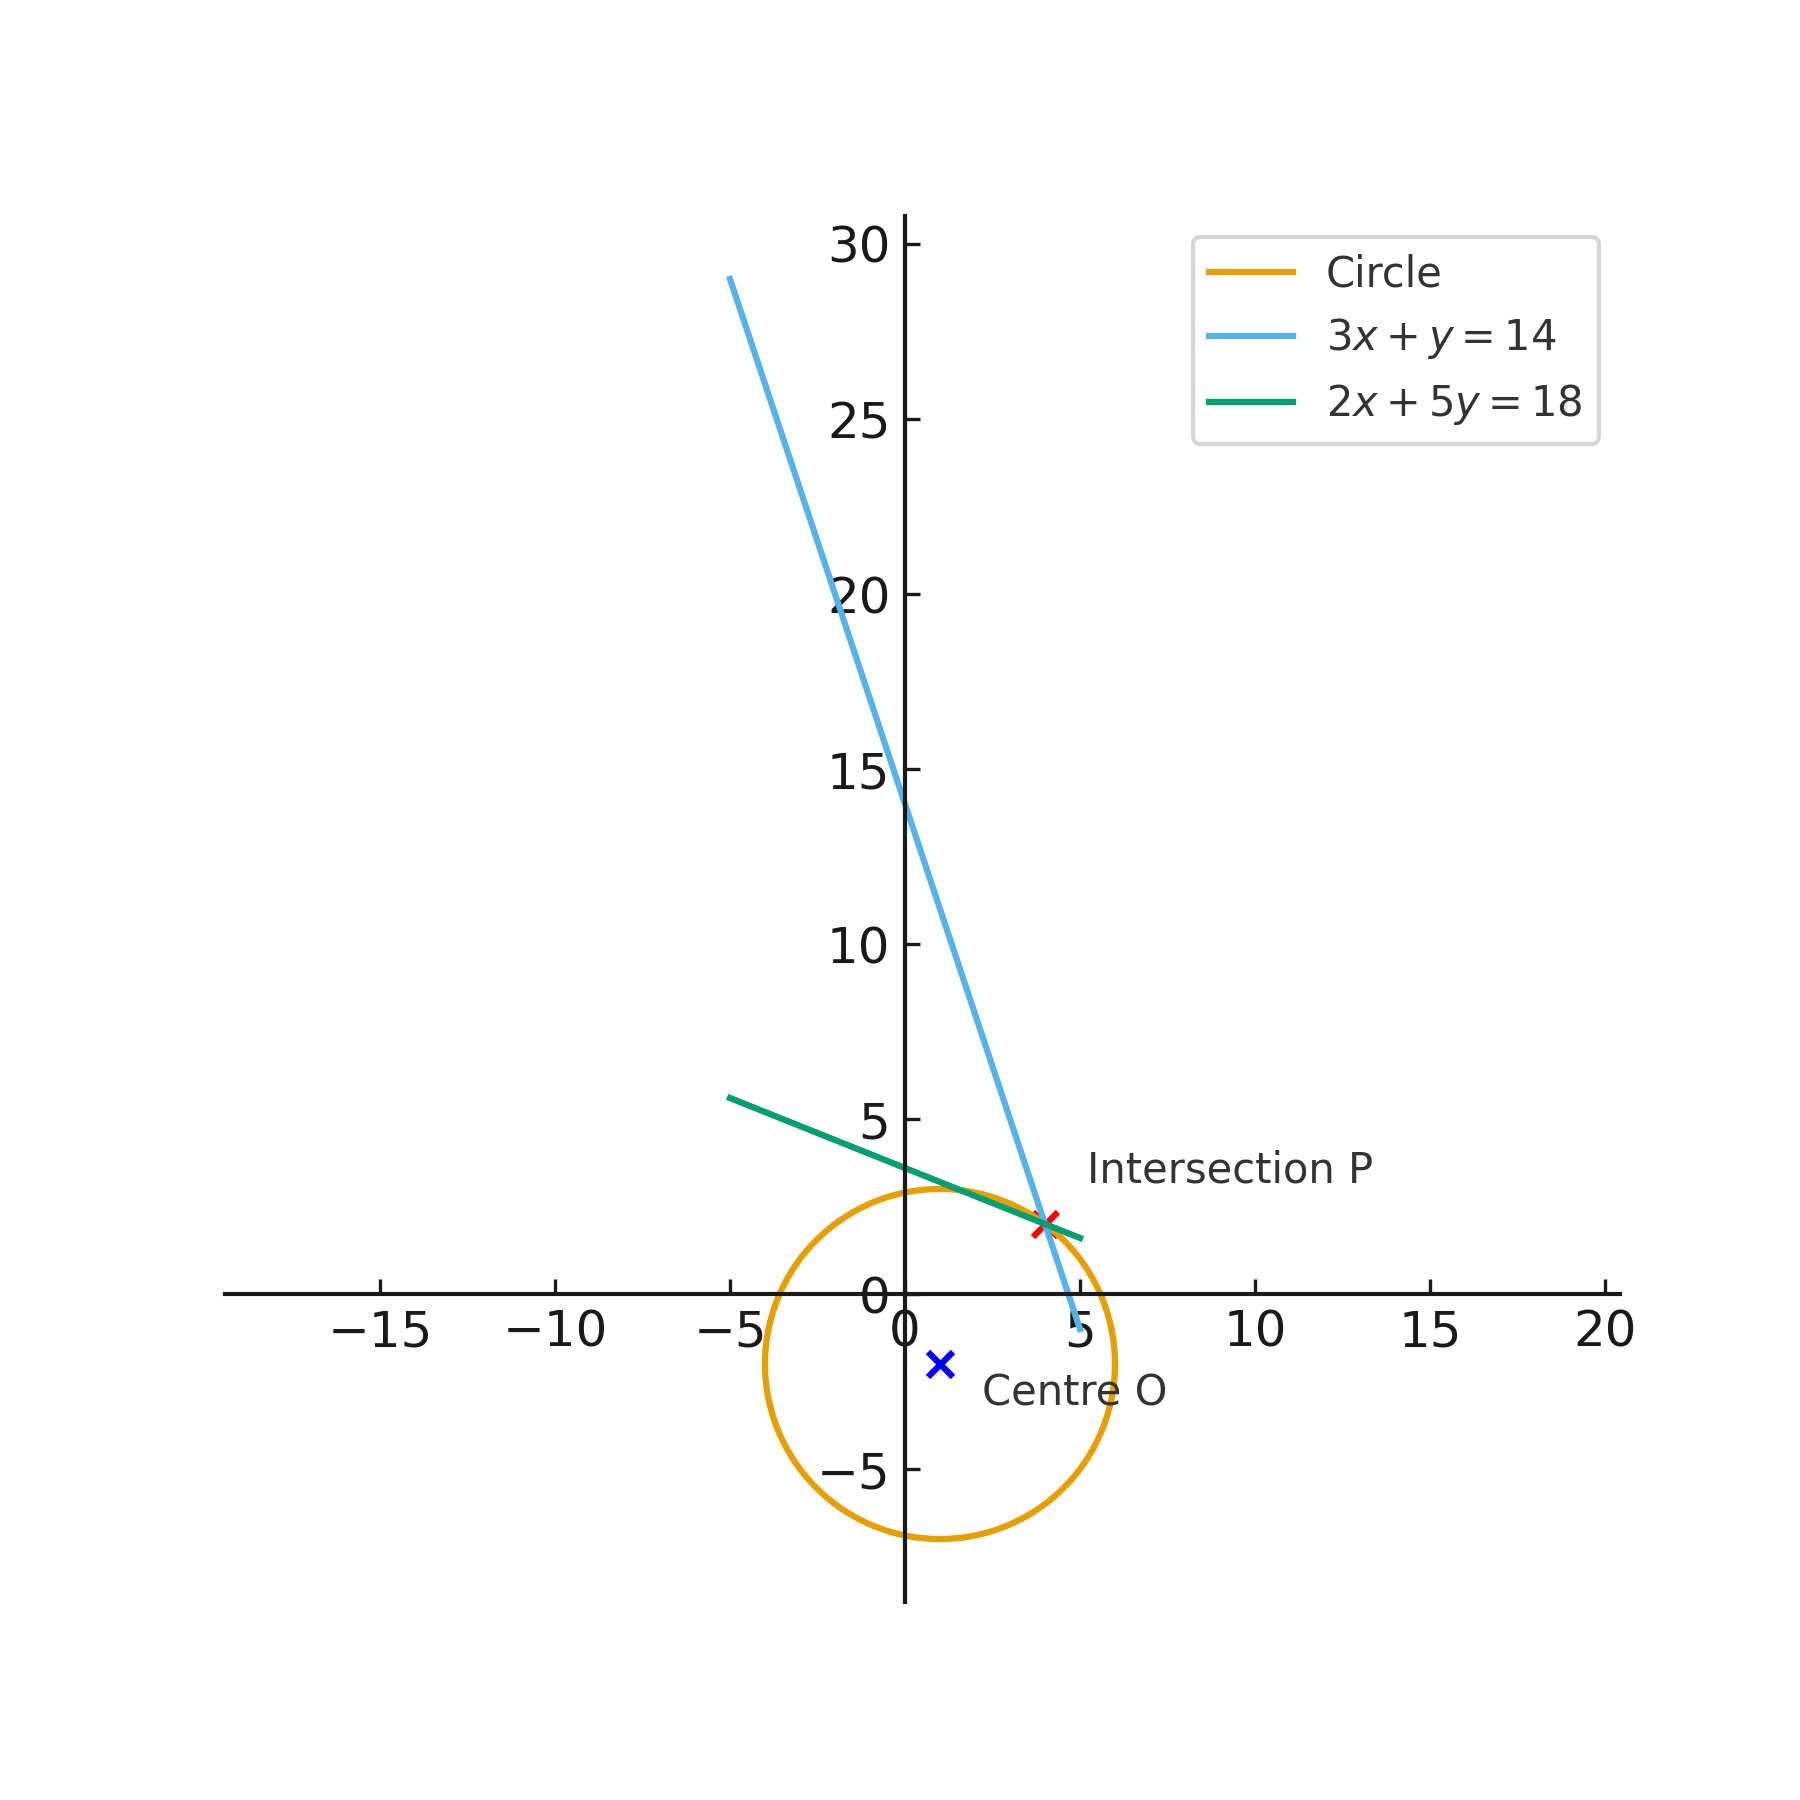
\includegraphics[width=\columnwidth, height=0.8\textheight, keepaspectratio]{figs/circle_question.png}     
\end{frame}
\end{document}